\chapter{REVISÃO BIBLIOGRÁFICA}
\label{cap:fundamentacao-teorica}

Este capítulo aborda os seguintes temas: metodologias no ensino da matemática, conceito de ambientes virtuais de aprendizagem, o uso da gamificação aplicada em AVAs, e, por fim, o que está sendo 
desenvolvido por outros pesquisadores da área.

\section{Metodologias no Ensino da Matemática}

Ao longo da história, várias metodologias e abordagens matemáticas foram utilizadas visando a melhoria do ensino. Segundo \citeonline{hammes2003tendencias}, algumas delas foram aula expositiva, 
resolução de problemas, modelagem matemática, e o uso de computadores. Nas seções a seguir, descreveremos cada uma delas.

\subsection{Aula expositiva}

Em uma aula expositiva, o professor comumente faz uma revisão da aula anterior, apresenta o novo conteúdo e passa aos alunos uma 
série de exercícios de fixação. Esse novo conteúdo é apresentado de forma oral ou escrita, sem levar em consideração o conhecimento 
prévio dos estudantes nem tempo para perguntas. Essa é, sem dúvida, uma das mais utilizadas e antigas metodologias existentes. Durante 
o século passado, aulas expositivas foram o único processo empregado em sala de aula pelos professores. Dessa forma, a aula expositiva pode 
ser considerada cansativa e desinteressante, já que o aluno não participa do processo de ensino  \cite{hammes2003tendencias}. Por outro 
lado, \'e uma das mais econômicas, flexível, proporciona que professor e alunos fiquem frente a frente com o conteúdo, além de ser um dos 
meios mais rápidos para atingir os objetivos de transmissão de determinados conteúdos \cite{marconteorias}. Para 
\citeonline{de1996gerencia}, essa abordagem possui diversos problemas, a escola tradicional não somente está desatualizada para atender às 
necessidades crescentes da sociedade contemporânea, como também apresenta algumas características que inibem o desenvolvimento do potencial 
de criação dos alunos:

\begin{alineascomponto}
\item Destaca-se a incompetência, a ignorância e a incapacidade do aluno, deixando de assinalar os talentos e habilidades de cada um; 
\item O ensino voltado para o passado, em que se enfatiza a reprodução e a memorização do conhecimento;
\item Desconsidera-se a imaginação e a fantasia como dimensões importantes da mente;
\item Exercício de resposta única, em que se cultua o medo do erro e do fracasso;
\item A obediência, dependência, passividade e conformismo são os traços mais cultivados;
\item Descaso em cultivar uma visão otimista do futuro;
\item As habilidades cognitivas são desenvolvidas de forma limitada;
\end{alineascomponto}

Autores como \citeonline{lopes1995aula}, defendem que a aula expositiva ``pode ser transformada em uma atividade dinâmica, participativa e 
estimuladora do pensamento critico do aluno''. Uma alternativa descrita por \citeonline{lopes1995aula} é transformar a aula 
expositiva em uma aula expositiva dialógica. Essa forma de aula expositiva utiliza o diálogo entre professor e aluno para estabelecer 
uma relação de intercambio de conhecimentos e experiências \cite{lopes1995aula}. De acordo com \citeonline{freire1982educaccao}, o 
ensino dialógico se contrapõe ao ensino autoritário, transformando  a  sala  de  aula  em  ambiente  propicio  à  reelaboração  e 
produção de conhecimentos.


\subsection{Resolução de problemas}\label{resolucao_problemas}

A resolução de problemas deve ser entendida como uma oportunidade para o aluno obter novos conhecimentos e não apenas 
conhecimentos prontos que fazem parte da nossa história. Ela ajuda o aluno a desenvolver sua autonomia buscando as respostas 
para seus próprios questionamentos. \citeonline{fossa1998tendencias} ressaltam  que esta metodologia visa o desenvolvimento de 
habilidades metacognitivas, favorecendo a reflexão e o questionamento do aluno que aprende a pensar por si mesmo, levantando 
hipóteses, testando-as, tirando conclusões e até discutindo-as com os colegas.

Podemos distinguir, mais claramente, um problema de um exercício. ``Um problema matemático é uma situação que demanda a 
realização de uma sequência de ações ou operações para obter um resultado. Ou seja, a solução não está disponível de início, mas é
possível construí-la'' \cite{nacionais1998terceiro}. Segundo \apud[p.4]{silveira2001problema}{deresoluccao}, ``um problema matemático é toda
situação que requer a descoberta de informações matemáticas desconhecidas para a pessoa que tenta resolvê-lo e/ou a invenção de uma 
demonstração de um resultado matemático dado. O fundamental é que o resolvedor conheça o objetivo a chegar, mas só estará enfrentando um
problema se ele ainda não tem os meios para atingir tal objetivo''. 

Como exemplo de problemas, apresentamos a seguinte situação envolvendo uma equação do 2º grau: \textit{Duzentas e quarenta figurinhas devem 
ser repartidas por um grupo de meninos, mas na hora de reparti-las 5 meninos não apareceram para pegar as suas figurinhas. Por causa disso, 
cada menino recebeu 8 figurinhas a mais. Quantos meninos receberam figurinhas?}

Para resolver este problema será necessário que o aluno traduza o enunciado para a linguagem matemática apropriada $\frac{240}{x} + 8 = 
\frac{240}{x-5}$, realizando manipulações algébricas para chegar à expressão $8x^{2}-40x-1200=0$ (ou $x^{2}-5x-150=0$). Após estes 
passos, o aluno poderá utilizar algum procedimento padronizado para a resolução, como por exemplo, a aplicação da fórmula de Bhaskara.

\citeonline{soares2001metodologia} acreditam que a utilização da resolução de problemas na pr\'atica educativa da matemática \'e
uma metodologia que deve merecer atenção por parte de todos professores. Pois \'e a partir deles que se pode envolver o aluno em situações 
da vida real, motivando-o para o desenvolvimento do modo de pensar matemático. Segundo eles, a resolução de um problema 
``exige uma certa dose de iniciativa e criatividade aliada ao conhecimento de algumas estratégias''. Um bom problema deve ser 
desafiador, mas possível de ser resolvido, real, interessante e que propicie várias estratégias de solução. Portanto, como se pode 
perceber, o número de variáveis envolvidas na resolução de problemas é grande, já que o ato de resolver não se relaciona apenas 
com o conhecimento em si. Outros fatores como a intuição, a criatividade, a perspicácia, a ansiedade, as frustrações etc, também interferem 
na atividade de resolver problemas, contribuindo para diferenciar as pessoas umas das outras \cite{mirian2001resolucao}. 

\subsection{Modelagem Matemática}

De acordo com \citeonline[p.~16]{bassanezi2002ensino}, ``[...] a modelagem consiste na arte de transformar situações da realidade em 
problemas matemáticos cujas soluções devem ser interpretadas na linguagem do mundo real''. \citeonline{biembengut1990modelaccao} acredita 
que a Modelagem está ligada \`a noção de trabalho de projeto. Segundo o autor, trata-se em dividir os alunos em grupos, os quais devem 
eleger temas de interesse para serem investigados por meio da matemática, contando com o acompanhamento do professor. Nas metodologias 
anteriores, o processo de ensino é deflagrado pelo professor. Na Modelagem Matemática, o processo é compartilhado com o grupo de 
alunos, pois sua motivação advém do interesse pelo assunto.

A Modelagem Matemática é uma metodologia que busca proporcionar ao aluno uma visão prática do conhecimento teórico aprendido na 
sala de aula, através de problemas de ordem prática ou de natureza empírica \cite{fossa1998tendencias}. \citeonline{barbosa2001modelagem} 
destaca alguns aspectos importantes a cerca dessa metodologia:

\begin{itemize}
	\item Maior interesse do(s) grupo(s) - O fato de o grupo compartilhar o processo de ensino, isto é, escolher aquilo que gostaria 
 de estudar, ter a oportunidade de se manifestar, de discutir e propor, desenvolve o interesse de cada grupo e dos grupos.
	\item Interação maior no processo de ensino e de aprendizagem - Para a aprendizagem, o procedimento gerado a partir do interesse do 
grupo ou dos grupos, parece resultar em ganho, pois o grupo ou os grupos de alunos trabalham com aquilo que gostam, aquilo que para 
eles apresenta significado, por isso tornam-se corresponsáveis pela aprendizagem.
	\item Demonstração de uma forma diferenciada de conceber a educação e, em consequência, a adoção de uma nova postura do professor. 
\end{itemize}

Na medida em que alunos e professores ``escolhem'' um tema gerador e o professor prop\~oe um determinado estudo, se poss\'ivel 
com um apelo social, os alunos buscam levantar informa\c{c}\~oes, organiz\'a-las, elaborar estratégias de a\c{c}\~ao, estimar e 
verificar resultados obtidos, entre outras a\c{c}\~oes. Mesmo que o problema inicial tenha uma origem n\~ao matem\'atica, o aluno v\^e 
obrigado a utilizar a l\'ogica, fazer uso de ideias, conceitos do campo matem\'atico para obter uma solu\c{c}\~ao para o assunto pesquisado 
\cite{silva2007modelagem}. \'E importante ressaltar que \'e muito difícil executar essa metodologia na pr\'atica, pois exige uma maior 
capacidade do aluno de solucionar problemas, trabalhar em grupo, saber pesquisar, ser pontual na entrega das tarefas, ser criativo, 
cumprir as metas, entre outros motivos.

\subsection{O Uso de Computadores}

A aprendizagem mediada por computadores surgiu em 1960 na Universidade de Illinois com o projeto PLATO (Programmed Logic for Automatic Teaching Operations)\cite{bitzer1961plato}, que deu origem ao primeiro sistema de ensino assistido por computador, o qual permitia a criação e apresentação de materiais sobre gram\'atica (passar um verbo para o passado, reescrever um substantivo no plural, etc.) com revisão automática. De acordo com \citeonline{woolley1994plato}, PLATO apoiou inicialmente apenas uma única sala de aula com 20 alunos, até que em 1972, o sistema migrou para uma nova geração de \textit{mainframes} que acabaria por apoiar milhares de terminais gráficos distribuídos em todo o mundo. O principal fator motivador para a introdução do computador na educação, segundo \citeonline{silva2009ambiente}, foi o surgimento no final do século XX de um conhecimento baseado em simulação, característico da cultura informática, o que fez com que o computador fosse visto como  um recurso didático  indispensável.

Os benefícios da utilização do computador como um instrumento de ensino e aprendizagem, de acordo com \citeonline[p.12]{almeida2000proinfo}, referem-se a sua utilização como ``uma máquina que 
possibilita testar ideias ou hipóteses, que levam à criação de um mundo abstrato e simbólico, ao mesmo tempo em que permite introduzir diferentes formas de atuação e interação entre as pessoas''. Já a 
principal associação de professores de matemática dos Estados Unidos (NCTM), diz que ``a tecnologia é essencial no ensino e 
na aprendizagem da Matemática'' e ``influencia a Matemática que é ensinada e melhora a aprendizagem dos alunos'' permitindo que estes se concentrem ``nas decisões a tomar, na reflexão, no raciocínio e 
na resolução de problemas''. \cite[p.26]{melo2007principios}.

Quando se fala no uso das Tecnologias da Informação e Comunicação (TIC) como um mediador para o processo de ensino e aprendizagem, muitas vezes, acaba-se esquecendo do papel do professor nesse 
processo. Num mundo em que há uma grande variedade de formas de utilização das TIC para apoio a educação, cabe ao professor decidir como e quando utilizar essas tecnologias e quais s\~ao formas 
mais eficazes para sua utilização levando em consideração os conteúdos que serão ofertados. Para isso, o professor necessita mudar sua metodologia de ensino, e isso pode resultar em problemas, já 
que, assim como afirmam \citeonline[p.~96]{bitner2002integrating}:

\begin{citacao}
``Adultos não mudam facilmente. Mudança de qualquer tipo traz medo, ansiedade e preocupação. A utilização da tecnologia como uma ferramenta de ensino e aprendizagem na sala de aula faz isso em um grau ainda maior, uma vez que envolve tanto mudanças nos procedimentos de sala de aula e o uso de tecnologias muitas vezes desconhecidas. Os responsáveis por pedir aos professores para usar a tecnologia no currículo devem estar cientes de que existem medos e preocupações.'' \cite[p.~96, Tradução Livre]{bitner2002integrating}.
\end{citacao}

Os problemas com a inserção do computador na educação podem ser ainda maiores, tendo em vista que muito se cogita sobre seu uso no ensino ser a solução para muitos dos problemas da educação, sendo que muitos desses problemas não podem encontrar uma solução nas tecnologias digitais \cite{silva2009ambiente}. Um dos fatores que pode influenciar negativamente no processo de aprendizagem mediada por computador é o domínio do computador pelo aluno, tendo em vista que sua rapidez de evolução assim como sua própria complexidade, torna essa tarefa muito difícil de ser alcançada.

\section{Ambientes Virtuais de Aprendizagem}

O surgimento de Ambientes Virtuais de Aprendizagem deu-se logo após o surgimento da internet nos anos 90. Nessa mesma época, novas ferramentas e produtos foram desenvolvidas para explorar os benefícios que a rede mundial de computadores trouxe \cite{oleary2002virtual}.

Para \citeonline{valentini2010aprendizagem}, um Ambiente Virtual de Aprendizagem é um espaço social, constituído de interações cognitivo-sociais sobre (ou em torno de) um objeto de conhecimento no qual as pessoas interagem, mediadas pela linguagem da hipermídia, visando o processo de ensino-aprendizagem.

Geralmente, os AVAs possuem algumas características que os distinguem de outros tipos de sistemas de softwares. Segundo \citeonline{oleary2002virtual}, algumas dessas características são:
\begin{alineascomponto}
    \item a comunicação entre tutores e alunos - por exemplo, email, fórum de discussão e bata-papo virtual;
    \item a auto-avaliação e avaliação sumativa - por exemplo, avaliação de múltipla escolha com automatizada marcação e feedback imediato; 
    \item entrega de recursos de aprendizagem e materiais - por exemplo, através do fornecimento de notas de aula e materiais, imagens e clips de vídeo;
    \item áreas do grupo de trabalho compartilhados - possibilita os usuários compartilharem arquivos e se comunicarem;
    \item suporte para estudantes - possibilita a comunicação entre os tutores e seus estudantes, fornecimentos de materiais didáticos e alguma forma de tirar as dúvidas dos alunos;
    \item gestão e acompanhamento dos estudantes - sistema de autenticação para permitir que apenas estudantes tenham acesso aos cursos;
    \item ferramentas para o estudante - por exemplo agendas e calendários eletrônicos;
    \item aparência consistente e personalizável - uma interface padrão de fácil utilização, permitindo personalização, mas com um modo de utilização básico.
\end{alineascomponto}

\citeonline{carvalho2013ambiente} afirma que AVAs integram funcionalidades de comunicação e partilha de informações e isso 
permite aceder à aprendizagem de uma forma flexível; em qualquer espaço(\textit{anywhere}) e em qualquer hora (\textit{anytime}). 
O autor complementa que:

\begin{citacao}
``Um AVA deve, por um lado, enfatizar a aprendizagem através da integração de ferramentas interativas e comunicativas, da 
partilha de conteúdos multimédia, do alojamento de trabalhos e projetos, da integração de ferramentas de aprendizagem colaborativa, 
e por outro, deve proporcionar estratégias que potenciem a participação ativa e significativa dos alunos, abranger possibilidades 
didáticas de aprendizagem individual e em grupo, criar novos acessos a websites como forma de enriquecer o conhecimento, possuir 
ferramentas de controlo de acesso e registro de utilizadores e de gestão de grupos de trabalho'' \cite[p.~41]{carvalho2013ambiente}. 
\end{citacao}

Muito se discute sobre as vantagens e desvantagens da utiliza\c{c}\~ao de AVAs na Educa\c{c}\~ao a Dist\^ancia (EAD). Entre as vantagens, 
destacam-se a acessibilidade a fontes inesgotáveis de assuntos para pesquisas, páginas educacionais específicas para a pesquisa escolar, 
comunicação e interação com outras escolas, estímulo para pesquisas a partir de temas previamente definidos ou a partir da curiosidade dos 
próprios alunos, estímulo ao raciocínio lógico, troca de experiências entre professores/professores, aluno/aluno e professor/aluno, dentre 
outras \citeonline{tajra2001ferramentas}. Entre as desvantagens, citam-se a incapacidade dos estudantes de auto-agendar e regular o 
desempenho. Estudantes que carecem de motivação e auto-disciplina tipicamente lutam mais em um AVA do que em uma sala de aula 
tradicional. Não há professores e colegas em posição de oferecer lembretes regulares sobre tarefas, projetos e testes. A interação limitada 
do tutor e o isolamento de um grupo de aprendizagem são também desvantagens. Os tutores normalmente tentam se comunicar através de e-mail 
ou pelas ferramentas do AVA. No entanto, é mais difícil garantir uma escuta adequada e compreensão a distância. Além disso, leva mais tempo 
para interação e feedback através de ferramentas virtuais do que face-a-face. O isolamento social pode ser desafiador 
para os alunos que desenvolvem a interação diária com os colegas e o conforto informal que vem com um ambiente de sala de aula tradicional.

\section{Gamificação}

Ao longo da história, buscamos metodologias inovadoras para auxiliar a educação. Uma das metodologias que mais diferem do tradicional método de ensino é a utilização de jogos para o ensino e aprendizagem. 

Surgiu em 2002, por meio de Nick Pelling, programador de computadores e inventor britânico, o termo Gamificação. \citeonline{fardo2013gamificaccao} define a Gamificação como o emprego de conceitos e 
técnicas criadas e utilizadas em jogos para auxiliar na educação. Alguns exemplos s\~ao:

\begin{alineascomponto}
	\item Sistema de Pontos: são abertos, diretos e motivacionais, permitindo a utilização de vários tipos diferentes de pontuação, de acordo com o objetivo proposto.
	\item Medalhas e Conquistas: tratam-se de uma representação visual de alguma realização/conquista do usuário no sistema. Os usuários querem receber medalhas dentro de um ambiente por diversos 
 motivos, para muitos, o objetivo é a experiência agradável de receber a medalha ou por “colecionar” medalhas.
	\item Desafios e Missões: são os elementos que orientam os usuários sobre as atividades que devem ser realizadas dentro de um sistema. É importante que existam desafios 
para os usuários completarem, pois isso fará com que exista algo interessante para ele realizar enquanto interage com o sistema.
	\item N\'iveis: indicam o progresso do usuário dentro do sistema. 
	\item Rankings: seu propósito principal é a comparação entre os jogadores/usuários envolvidos.
	\item Personalização: permite o usuário transformar e personalizar itens que compõem o sistema de acordo com seu gosto, promovendo motivação, engajamento, sentimento de posse e controle sobre 
o sistema. 
\end{alineascomponto}

Para \citeonline{halliwell2013gamification}, o objetivo da Gamificação não é transformar tudo em um jogo, mas sim, encontrar a diversão, encontrar os aspectos `jogáveis' de um problema, quaisquer que 
sejam, e usá-los para criar um ambiente que mova as pessoas um pouco mais em direção a um objetivo que tenham criado. Um exemplo bem interessante do uso de gamificação é o Duolingo\footnote{O 
Duolingo é uma plataforma para ensino de idiomas gratuito, dispon\'ivel em \url{www.duolingo.com} } \cite{von2013duolingo}, uma plataforma online de aprendizagem em línguas que trabalha com o 
conceito de conhecimento coletivo e voluntário. No Duolingo, usuários podem ganhar pontos com as respostas corretas e lições completadas, assim como perder pontos a cada resposta incorreta. O mesmo 
ainda atribui status de reconhecimento de acordo o conhecimento obtido durante o jogo. Veja mais na 
\autoref{trabalho_relacionados_duolingo}.

A Gamificação ainda \'e muito nova e possui potencialidades de aplica\c{c}\~ao em diversas áreas, pois a linguagem e metodologia dos 
\textit{games} s\~ao bastante populares, eficazes na resolução de problemas e aceitas naturalmente pelas atuais gera\c{c}\~oes que 
cresceram interagindo com esse tipo de entretenimento. Dessa forma, a gamificação se justifica a partir de uma perspectiva sociocultural 
\cite{fardo2013gamificaccao}. Por ser um fen\^omeno emergente, existem poucos relatos de sua utiliza\c{c}\~ao em processos educacionais, 
devido ao fato de que os educadores precisam dominar bem essa linguagem para serem capacitados para aplicar em seus projetos 
\cite{fardo2013gamificaccao}. Por isso, aplic\'a-la na educa\c{c}\~ao pode impactar de forma inesperada os processos de ensino e 
aprendizagem. Al\'em de haver um risco de ser empregada de forma incorreta e equivocada, refor\c{c}ando ainda mais os problemas enfrentados 
no ensino tradicional, como por exemplo, uma valoriza\c{c}\~ao maior na nota obtida do que na pr\'opria 
aprendizagem. \citeonline{fardo2013gamificaccao} explica que isso pode acontecer se, ao aplicarmos a gamifica\c{c}\~ao, utilizarmos
apenas as mecânicas mais básicas dos games e com isso construirmos somente um sistema mais complexo de pontuação, por exemplo.   

\section{Trabalhos Relacionados}
\label{cap:trabalhos-relacionados}

Os Ambientes Virtuais de Aprendizagem vêm sendo utilizados na educação, principalmente como uma ferramenta mais dinâmica, se comparados \`as metodologias de ensino tradicionais, e são de 
grande potencial na área da educação. Existem diversas pesquisas voltadas a aplicação de AVAs para apoiar o processo de ensino-aprendizagem e, em especial, a Matemática se destaca entre elas.

\subsection{\textit{The one world schoolhouse: Education reimagined}}
Em um trabalho iniciado em 2006, \citeonline{khan2012one} fundou a chamada Khan Academy\footnote{Plataforma de aprendizagem disponível em: \url{www.khanacademy.org}}, organização educacional que tem 
por objetivo oferecer exercícios, vídeos de instrução e um painel de aprendizado personalizado que habilita os estudantes a aprender no seu próprio ritmo dentro e fora da sala de aula. Em sua 
plataforma, são abordados assuntos como matemática, ciência, programação de computadores, história, história da arte e economia, entre outros \cite{khan2012one}.

No ambiente, o desempenho do estudante é representado por medalhas. De acordo com o site da organização, medalhas e insignias estimulam o aprendizado de maneira lúdica. As estatísticas mostram o 
quanto de trabalho o estudante está fazendo a cada dia, o quanto o estudante está focado em áreas de habilidades e tópicos e as habilidades que o estudante concluiu. Com os relatórios gerados pela 
plataforma, o tutor pode acompanhar todos os passos do estudante.

Durante uma conferência TED\footnote{É uma série de conferências realizadas na Europa, Ásia e Américas pela fundação Sapling com o objetivo de disseminar ideias que podem mudar o mundo.} em 2011, 
denominada \textit{Salman Khan: Let's Use Video to Reinvent Education} \cite{tedtalk2011reinvend}, Khan fala sobre o funcionamento da plataforma e também do provável motivo do seu sucesso. Segundo 
\citeonline{tedtalk2011reinvend}, o diferencial da plataforma está em dois pontos importantes, a aprendizagem auto-ritmada e nos dados fornecidos aos tutores sobre o aprendizado de seus estudantes. 

Em relação a aprendizagem auto-ritmada, Khan afirma que:
\begin{citacao}
``Então quando fala-se em aprendizagem auto-ritmada, isso faz sentido para todo mundo – na chamada aprendizagem diferenciada – mas é meio maluco quando você vê isso na sala de aula. Porque toda vez 
que fizemos isso, em cada sala de aula que fizemos, repetidas vezes, depois de cinco dias nisso, há um grupo de garotos que está adiantado e há outro grupo de garotos um pouco atrás. E num modelo 
tradicional, se você fizesse uma avaliação pontual, diria: ``Esses são garotos inteligentes, aqueles são garotos lerdos. Talvez eles devessem ser acompanhados de forma diferente. Talvez devêssemos 
coloca-los em salas diferentes.'' Mas quando você deixa cada aluno trabalhar em seu próprio ritmo – e vemos isso repetidas vezes – você vê alunos que tomam um tempo extra em um conceito ou outro, mas 
uma vez que adquirem esse conceito, eles apenas vão adiante. E assim os mesmos garotos que você pensava que eram lerdos semanas atrás, agora você pensa que são inteligentes. E vemos isso repetidas 
vezes. E isso faz você se perguntar quantos estereótipos que talvez vários de nós recebemos eram apenas devido a uma coincidência de tempo'' \cite[13:29, Tradu\c{c}\~ao 
Livre]{tedtalk2011reinvend}.
\end{citacao}.


\citeonline{tedtalk2011reinvend} também fala sobre a importância dos dados fornecidos pelos tutores:
\begin{citacao}
``[...]. Nosso paradigma é armar os professores com a maior quantidade de dados possível – dados que, em quase qualquer outro campo, são esperados, se você trabalha com finanças ou propaganda ou 
fabricação. E assim o professores podem realmente diagnosticar o que está errado com os alunos de maneira que podem fazer suas interações mais produtivas possível. Agora os professores sabem 
exatamente o que os alunos têm feito, quanto tempo eles gastam todo dia, a quais vídeos assistiram, quando pausaram os vídeos, o que fez que parassem de ver, quais exercícios estavam fazendo, no que 
eles estavam se focando? [...]'' \cite[12:26, Tradu\c{c}\~ao Livre]{tedtalk2011reinvend}.
\end{citacao}

O trabalho de \citeonline{khan2012one}, assim como o apresentado nesta monografia, apresenta o uso de um AVA para auxiliar na educação. Dessa forma, esse trabalho servirá como referência para abordar 
o uso da aprendizagem auto-ritmada na educação matemática, assim como para definir as informações que deverão ser apresentadas aos tutores sobre a evolução da aprendizagem de seus estudantes na 
plataforma fruto deste trabalho. Contudo, os vídeos ``que fizeram da Khan Academy tão popular'' não fazem parte desse trabalho.

O aspecto mais importante a se considerar aqui está na forma como as duas plataformas lidam com Obstáculos Epistemológicos. Segundo \citeonline{bachelard1996formaccao}, durante o ato do conhecimento, 
ocorrem ``lentidões e conflitos'' que levam o estudante a parar diante do problema. A esta ``inércia'' é que foi relacionado o conceito. Na metodologia criada por \citeonline{khan2012one}, quando a 
plataforma é aplicada dentro da sala de aula, o professor pode identificar através da ferramenta, os estudantes que estão com esses obstáculos e o mesmo pode intervir para ajudar esses estudantes a 
superar essa barreira. No trabalho apresentado aqui, essa barreira será superada quando o sistema, ao identificar o obstáculo enfrentado, indicar ao estudante a exist\^encia desse obst\'aculo e o(s) 
conte\'udo(s) que ele possui defici\^encia (causador(es) da barreira) para ele assim poder pausar o conte\'udo que est\'a estudando e voltar a estudar o(s) conte\'udo(s) mais b\'asicos que o sistema 
indicar. Por esse método o  estudante, ao enfrentar um obst\'aculo na aprendizagem, saber\'a quais os conte\'udos estudados anteriormente foram os causadores desse obst\'aculo e poder\'a, dessa 
forma, focar seus estudos nesses conte\'udos para superar essa barreira.

\subsection{\textit{ActiveMath: A generic and adaptive web-based learning environment}}

O projeto ActiveMath visa apoiar a aprendizagem verdadeiramente interativa, exploratória, e assume que o estudante deve ser responsável por seu aprendizado. Portanto, uma relativa liberdade para 
navegar através de um curso e para as escolhas de aprendizagem lhes é dada e, por padrão, o modelo de usuário é inspecionável e modificável \cite{melis2001activemath}. 
\citeonline{melis2001activemath} afirmam que a maioria dos sistemas tutores inteligentes não contam com uma escolha de adaptação de conteúdos e isso, segundo \citeonline{melis2001activemath}, pode 
influenciar quando o público-alvo for alunos de faculdades e universidades, já que, diferentemente das escolas de ensino fundamental,  um mesmo assunto é ensinado de forma diferente para diferentes 
grupos de utilizadores e em contextos diferentes \cite{melis2001activemath}.

Para conseguir um ambiente dinâmico de aprendizagem, ActiveMath utiliza regras pedagógicas que definem em quais momentos determinadas funcionalidades do sistema estarão disponíveis, em que ordem os 
conteúdos serão apresentados para os alunos e como os mesmos deverão ser apresentados. O trabalho referido,  assim como o desenvolvido por \citeonline{khan2012one} descrito anteriormente, descreve a 
criação de um AVA, o mesmo utiliza tamb\'em técnicas que permitem a geração dinâmica de cursos para os alunos.

O trabalho desenvolvido por \citeonline{melis2001activemath} apresenta um subsistema de exerc\'icios que suporta diagn\'osticos de erros e equ\'ivocos dos estudantes, que 
gera estrat\'egias tutoriais configur\'aveis para o \textit{feedback}. Em nosso trabalho, quando o ambiente diagnosticar erros e equ\'ivocos frequentes cometidos pelos estudantes relacionados a 
um conte\'udo estudado anteriormente, o sistema alertar\'a ao estudante sobre uma poss\'ivel defici\^encia que ele possua e o orientar\'a a voltar a estudar o conte\'udo indicado.


\subsection{\textit{Duolingo: Learn a Language for Free while Helping to Translate the Web}}\label{trabalho_relacionados_duolingo}

Nesse trabalho desenvolvido por \citeonline{von2013duolingo}, \'e apresentado o Duolingo, uma plataforma de ensino de idiomas e tradu\c{c}\~ao autom\'atica de documentos. O ambiente funciona de 
maneira que os usuários progridam nas lições ao mesmo tempo que traduzem conteúdo real da internet. 

O método utilizado pela plataforma se caracteriza pela li\c{c}\~oes fragmentadas, pelas quais os 
alunos, atrav\'es do m\'etodo de repeti\c{c}\~ao, fixam o conte\'udo da língua estudada. \`A medida que o usu\'ario avan\c{c}a, ele progride em uma \'arvore de habilidades que o leva gradativamente 
ao fim do curso, enquanto oferece a op\c{c}\~ao de voltar atr\'as para refazer li\c{c}\~oes antigas que j\'a poderiam ter sidas esquecidas. Um estudo realizado na Universidade da Cidade de Nova York 
\cite{vesselinov2012duolingo} disse que 34 horas gastas no Duolingo igualou-se a um semestre de um curso de l\'inguas.

Uma das características mais marcantes dessa plataforma \'e quantidade de técnicas de Gamifica\c{c}\~ao empregadas. Possui sistema de pontua\c{c}\~ao, n\'iveis, rankings, miss\~oes, medalhas, 
personaliza\c{c}\~ao, entre outras. Assim como a plataforma desenvolvida por \citeonline{von2013duolingo}, o ambiente que desenvolveremos tamb\'em contar\'a com t\'ecnicas de Gamifica\c{c}\~ao que 
ser\~ao utilizadas para melhorar a experi\^encia do usu\'ario, assim como para motivar esses usu\'arios durante sua utiliza\c{c}\~ao do sistema.

\subsection{\textit{Resolução de problemas em ambientes virtuais de aprendizagem num curso de licenciatura em matemática na modalidade a distância}}

O trabalho desenvolvido por \citeonline{dutra2011resoluccao}, trata da utilização da metodologia de Resolução de Problemas (apresentada na \autoref{resolucao_problemas}) em um AVA com o objetivo de 
investigar as contribuições que essa jun\c{c}\~ao pode trazer para um curso de Licenciatura em Matem\'atica da Universidade Federal de Ouro Preto (UFOP). Para isso, 
o ambiente desenvolvido por \citeonline{dutra2011resoluccao} utiliza de fóruns semanais para discussão e resolução dos problemas, além de chats, utilizados ao final de algumas atividades, e um 
questionário final a ser respondido pelos alunos na última semana de aula.

Essa metodologia, segundo \citeonline{dutra2011resoluccao}, funciona atrav\'es dos seguintes passos:
\begin{alineascomnumero}
	\item A atividade é postada na Plataforma Moodle\footnote{``A  palavra  Moodle  referia-se  originalmente  ao  acrônimo:  `Modular Object-Oriented  Dynamic  Learning  Environment'(...).  Em  inglês  a  palavra Moodle é também um verbo que descreve a ação que, com frequência, conduz a resultados criativos, de deambular com preguiça, enquanto se faz com gosto o  que  for  aparecendo  para  fazer''. O  Moodle  deu  o  nome  a  uma  plataforma  de  e-learning,  de  utilização livre  e  código  fonte  aberto,  pela  mão  de  Martin  Dougiamas \cite{oro29585}.} no início da semana, pela manhã (segunda-feira).  Assim,  as  atividades  são  distribuídas  aos  alunos  para  que possam ler, interpretar e entender o problema. 
	\item Os  alunos  passam a  semana  postando  suas  resoluções  dos  problemas e discutindo-as no fórum com os colegas, por meio da Plataforma Moodle. 
	\item A  pesquisadora  observa,  incentiva  e  participa  do  processo  de discussão, ajuda nos problemas secundários, dando \textit{feedback} das resoluções postadas, respondendo e fazendo 
perguntas, tirando  dúvidas, acompanhando de perto as discussões entre os alunos no fórum.
	\item As impressões dos alunos sobre os problemas, no início da semana seguinte, e a formalização dos resultados são apresentadas nos chats semanais. Trata-se  de  uma  plenária  virtual  para  discutir  os  problemas,  finalizando-a  com  uma solução aceita por todos. 
	\item Uma resolução é postada na Plataforma Moodle, para todos os pesquisados, observando os conteúdos apresentados nos problemas. 
\end{alineascomnumero}

O trabalho apresentado aqui, assim como o desenvolvido por \citeonline{dutra2011resoluccao}, utiliza a Metodologia de Resolu\c{c}\~ao de Problemas para auxiliar no ensino de matem\'atica. Uma 
outra característica que as duas metodologias t\^em em comum \'e o uso de f\'oruns de discuss\~ao como ferramenta que propicia uma 
constru\c{c}\~ao coletiva de conhecimento, atrav\'es do compartilhamento do conhecimento.


\section{Considerações finais do cap\'itulo}

A plataforma que desenvolveremos faz uso da metodologia de resolução de problemas, possibilitando o aluno adquirir novos conhecimentos além daqueles estudados no momento. Por se tratar de um AVA, 
o mesmo possibilitará ao aluno uma maior interação com o professor e outros alunos, além da possibilidade de uma aprendizagem auto-ritmada. A aplicação da Gamificação no sistema, servir\'a para desenvolver  engajamento, participação, e comprometimento entre os usuários do sistema. 

Uma caracteristica importante em nossa plataforma, que a diferencia das demais citadas até momento, é a forma com ela lidará com as deficiências de aprendizado que os alunos enfretam ao longo de seus estudos. É possível, a partir de um item respondido incorretamente de um problema, identificar a deficiência do estudante. Por isso, é fundamental que no momento que o assistente estiver adicionando os itens do problema, ele possa escolher, para cada item incorreto, uma ou várias li\c{c}\~oes, indicando-lhes como supostas defici\^encias do estudante caso ele marque determinados itens. Na \autoref{fig:estrutura_problema}, ilustramos a estrutura dos problemas que são utilizados no ambiente. No problema, apenas o primeiro item é correto, os demais são incorretos. Os incorretos podem, ou não, indicar as deficiências que o aluno possua caso este conclua sua resposta marcando este determinado item. A medida que os erros do aluno forem se acumulando, pode ocorrer que os itens marcados incorretamente em suas respostas, indiquem deficiências que este aluno venha a ter.

\begin{figure}[H]
    \centering
    \Caption{\label{fig:estrutura_problema} Estrutura do Problema}	
    \UFCfig{}{
	\fbox{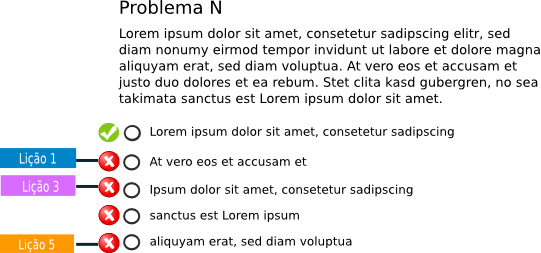
\includegraphics[width=8cm]{figuras/figura_estrutura_problema.png}}
    }{
      \Fonte{Do próprio autor.}
    }	
\end{figure}

Na \autoref{fig:ilustracao_aprendizagem}, ilustramos o nosso modelo de aprendizagem. Nesse modelo, cada conteúdo é fragmentado em lições, e durante o aprendizado dessas lições, pode ocorrer de alguns alunos ficarem para trás (Cena 1). Destes que ficaram para tráz, alguns podem vir a enfrentar obstáculos e não consiguam avançar para as próximas lições (Cena 2). Ao identificar isso, o sistema poderá identificar as lições que estes alunos possuem deficiência e lhe sugira voltar para refazer essas lições antes de continuar (Cena 3). Após o aluno refazer a  provável lição em que possui deficiência (Cena 4), este já estará hábito a superar o obstáculo e continuar com seu aprendizado (Cenas 5 e 6).

\begin{figure}[H]
    \centering
    \Caption{\label{fig:ilustracao_aprendizagem} Problema}	
    \UFCfig{}{
	\fbox{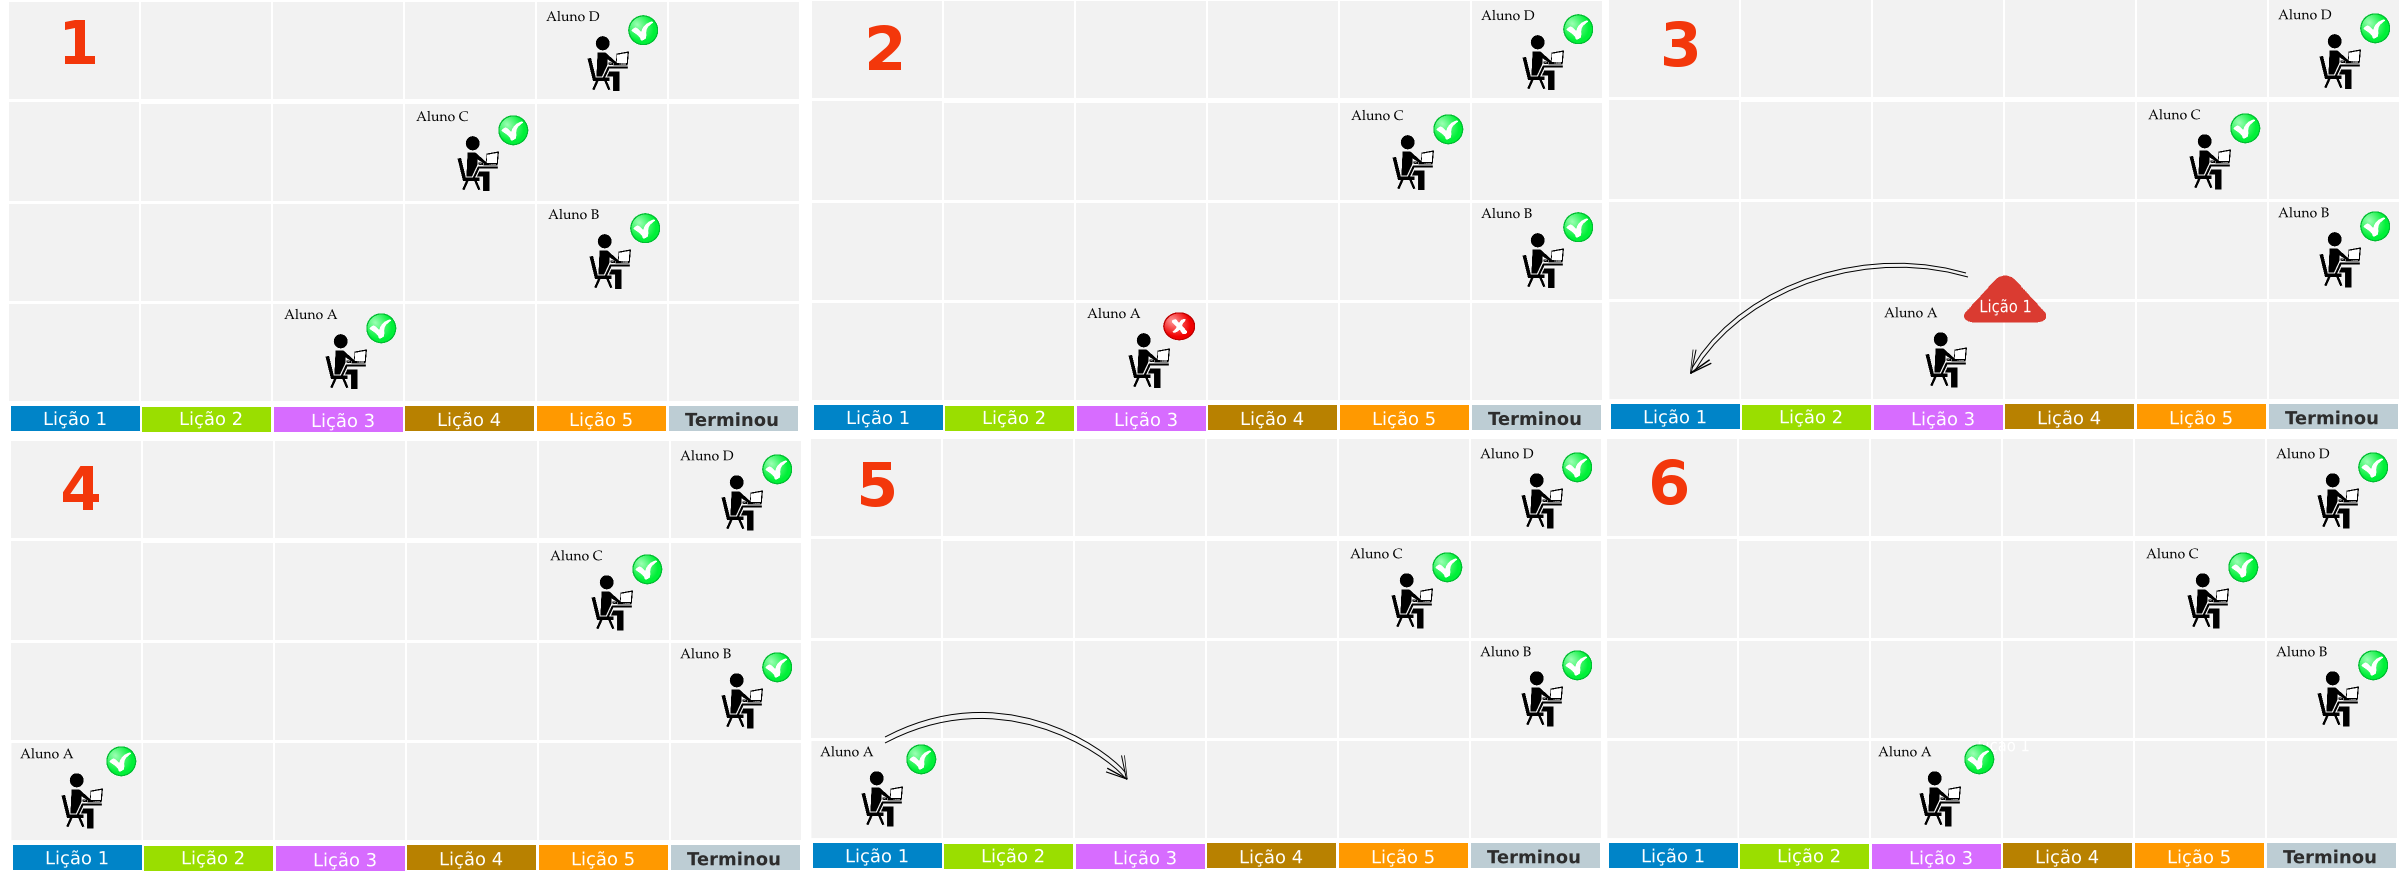
\includegraphics[width=\textwidth]{figuras/proposta.png}}
    }{
      \Fonte{Do próprio autor.}
    }	
\end{figure}